\documentclass[tikz,border=8pt]{standalone}
% Shared look for every TikZ diagram. Load with \input{../../tools/tikz-style.tex}
\usepackage[T1]{fontenc}
\usepackage{lmodern}
\renewcommand{\sfdefault}{lmr}  % diagrams use the same serif as the text
\usetikzlibrary{arrows.meta, positioning, shapes.geometric, calc, fit, backgrounds}
\definecolor{cblue}{HTML}{4C78A8}
\definecolor{corange}{HTML}{F58518}
\definecolor{cgreen}{HTML}{54A24B}
\definecolor{cred}{HTML}{E45756}
\definecolor{cpurple}{HTML}{B279A2}
\definecolor{cgrey}{HTML}{6B6B6B}
\tikzset{
  every picture/.style={font=\sffamily, line width=1.2pt},
  box/.style={draw=#1, fill=#1!12, rounded corners=4pt, align=center, inner sep=7pt, minimum height=1.1cm},
  box/.default=cgrey,
  arrow/.style={-{Stealth[length=3mm]}, draw=cgrey, line width=1.4pt},
  title/.style={font=\sffamily\bfseries\Large},
  note/.style={font=\sffamily\small, text=cgrey, align=center},
}
\AtBeginDocument{\hyphenpenalty=10000 \exhyphenpenalty=10000}

\begin{document}
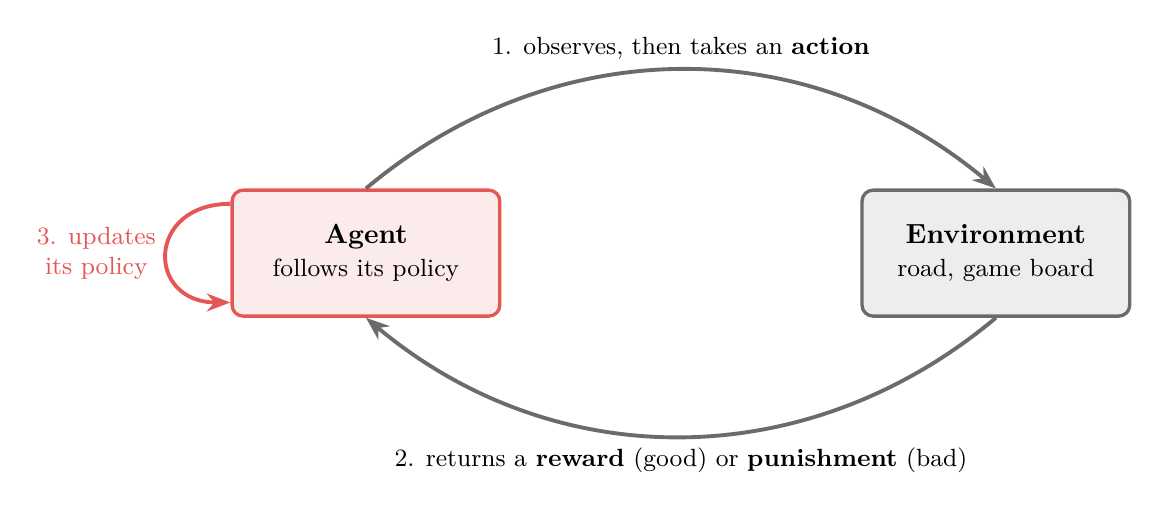
\begin{tikzpicture}
  \node[box=cred, minimum width=3.4cm, minimum height=1.6cm, font=\sffamily\bfseries] (agent) at (0,0) {Agent\\{\small\mdseries follows its policy}};
  \node[box=cgrey, minimum width=3.4cm, minimum height=1.6cm, font=\sffamily\bfseries] (env) at (8,0) {Environment\\{\small\mdseries road, game board}};
  \draw[arrow] (agent.north) to[out=40, in=140] node[note, above, text=black] {1. observes, then takes an \textbf{action}} (env.north);
  \draw[arrow] (env.south) to[out=-140, in=-40] node[note, below, text=black] {2. returns a \textbf{reward} (good) or \textbf{punishment} (bad)} (agent.south);
  \draw[arrow, draw=cred] (agent.160) to[out=180, in=180, looseness=2.2] node[note, left, text=cred] {3. updates\\its policy} (agent.200);
\end{tikzpicture}
\end{document}
